\documentclass{article}

\usepackage[utf8]{inputenc}
\usepackage[T1]{fontenc}
\usepackage[norsk,english]{babel}   %norsk først så engelsk, så engelsk blir prioritert
\usepackage{graphicx}
\usepackage{amsmath}
\usepackage{listings}
\usepackage{multicol}
\usepackage[margin=2cm]{geometry}
\usepackage{wrapfig}

%Definerer hyperlinker og dens farger
\usepackage{hyperref}
\hypersetup{
    colorlinks,
    citecolor=black,
    filecolor=black,
    linkcolor=blue,
    urlcolor=blue
}

%-----------------------------------

%Definerer farger til kodeeksemplene i PDF-en
\usepackage{color}

\definecolor{codegreen}{rgb}{0,0.6,0}
\definecolor{codegray}{rgb}{0.5,0.5,0.5}
\definecolor{codepurple}{rgb}{0.58,0,0.82}
\definecolor{backcolour}{rgb}{0.95,0.95,0.92}

\lstdefinestyle{mystyle}{
    backgroundcolor=\color{backcolour},
    commentstyle=\color{codegreen},
    keywordstyle=\color{magenta},
    numberstyle=\tiny\color{codegray},
    stringstyle=\color{codepurple},
    basicstyle=\footnotesize,
    breakatwhitespace=false,
    breaklines=true,
    captionpos=b,
    keepspaces=true,
    numbers=left,
    numbersep=5pt,
    showspaces=false,
    showstringspaces=false,
    showtabs=false,
    tabsize=2
}

\lstset{style=mystyle}

%------------------------------------

\setlength{\parindent}{0pt}
\setlength{\columnsep}{5mm} %column separation
\setlength{\columnsep}{10mm}

\setlength{\tabcolsep}{18pt}
\renewcommand{\arraystretch}{1.5}

\iffalse
If you want to change this temporarily, you can write:
\savegeometry{mydefaultgeometry}
\newgeometry{margin=3in}
And then later you can call:
\loadgeometry{mydefaultgeometry}
\fi

\begin{document}

\addtocounter{page}{0}

\title{Project 2 \\
      \large For the course FYS3150}
\date{\today \\
    \vspace{1mm}
    \large Week 37 - 40}

\author{Erik Grammeltvedt, Erlend Tiberg North and Alexandra Jahr Kolstad}

\maketitle

%\newpage

%------------Her starter skrivingen-----------------------------------------
\vspace{1cm}

\tableofcontents

\vspace{1cm}

%---------------------------------------
%\begin{multicols}{2}

\newpage
\clearpage

\vspace{2cm}

%----------Abstract-------------------------------
\vspace{1cm}

\section{Abstract} \label{sec:Abstract}

The overall goal of this project is to make an eigenvalue solver and to show its relevance by solving some quantum mechanical problems, but firstly by testing it for a simpler classical problem. In this project we are focusing on using the Jacobi method in order to find the eigenvalues and eigenvectors of a matrix.  As well as comparing it to imported eigenvalue and eigenvector solvers from armadillo to see witch method is most potent.


%--------------Introduction------------------------------
\vspace{1cm}

\section{Introduction} \label{sec:Introduction}

All programs are found at our \href{https://github.com/Erikbgram/Fys3150}{GitHub-repository}. \\

The versatility of many numerical methods are astounding and fundamentally important for humanities understanding of the world. For instance the method used in this problem starts out very basic but goes on to solve problems in the quantum mechanic realm with small variations to the code. This project focuses on numerical eigenvalue solvers or more specifically the Jacobi method. The article starts by describing how the one dimension beam problem can be simplified and discretized into a numerically solvable problem.

\begin{equation*}
  -\lambda u_i = \frac{-(-u_{i-1} + 2u_i - u_{i-1})}{h^2}
\end{equation*} \\

The problem in this project is divided into two parts: first we are going to look at a beam in the $y$-direction and secondly electrons in a three-dimensional harmonic potential. This is respectively a classical problem and a quantum mechanical problem. Both of these problems are eigenvalue problems, and will be solved with the Jacobi method implemented in our algorithm. We will compare the results from our algorithm with results of the Armadillo function \texttt{eig\_sym}. \\

Followed by the proof that the Jacobi method is useable because it does not change the eigenvectors, the project then explains basic quantum mechanics needed in order to see how the Jacobi method is applied in this project. Then an explanation to how we have implemented the Jacobi method is given in the program \texttt{jacobomethod.cpp}. Followed by the results showing that the Jacobi method is very slow compared to other eigenvalue and eigenvector solving methods that can be used, from for instance Armadillo. The conclusion to this project is that the Jacobi method is an inefficient method to solve eigenvalues, however the project demonstrates the power of such a solver and its many different applications. \\

This project is seperated into sections with some subsections. See table of contents for page number to the sections. In \nameref{sec:Theory} we will present essential theory to understand our problem, why we solve it and how we solve it. In \nameref{sec:Method} we will explain why we use the Jacobi algorithm to solve our problem. Furthermore it includes explanations to the unit tests we chose in our algorithm.
In \nameref{sec:Results} we will present the data and the plots generated in our programs, with a short explanation of what the results present. The section \nameref{sec:Discussion} is where we will consider our problem, and discuss why the two methods Jacobi method and the Armadillo function \texttt{eig\_sym} gives different computation times. After this we will conclude our findings in the section \nameref{sec:Conclusion}.
Finally we have the section \nameref{sec:Appendix} for additional information, such as derivations, comments and figures, tables or text, and the section \nameref{sec:References} for citing every reference in one place. \\

Our project consists of the files \texttt{jacobimethod.cpp} and \texttt{plot\_data.py}. \texttt{jacobimethod.cpp} is the main program for computing the Jacobi method, while \texttt{plot\_data.py} plots the data generated in \texttt{jacobimethod.cpp}, which is appended into \texttt{.txt}-files. The \texttt{.txt}-files in this project are \texttt{stats.txt}, \texttt{harmonic.txt} and \texttt{qdot.txt}.  \\


%--------------- Theory ------------------------------------
\vspace{1cm}

\section{Theory} \label{sec:Theory}

\subsection{Orthogonality of a unitary transformation} \label{sec:orthogonality}

Firstly we are going to prove that $\vec{w}_i = U \vec{v}_i$ is an orthogonal or unitary transformation that preserves the dot product and orthogonality. We start by multiplying $\vec{w}_j ^T$ with $\vec{w}_i$ to take the vector product, also called the dot product. If the vector product of these vectors is equal to $\delta_{ij}$, given by $\vec{v}_j ^T \vec{v}_i = \delta_{ij}$ in the exercise, then the dot product and orthogonality is preserved. In this exercise we assume that $U^T U = I$, where $I$ is the identity matrix, because this defines a unitary matrix $U$ which we compute with in this exercise. \\

The vector product is calculated as followed:

\begin{align*}
  \vec{w}_j ^T \vec{w}_i &= (U \vec{v})^T U \vec{v}_i \\
  &= \vec{v}_j ^T U^T U \vec{v}_i \\
  &= \vec{v}_j ^T \vec{v}_i \\
  &= \delta _{ij}
\end{align*}

The vector product of $\vec{w}_j ^T$ and $\vec{w}_i$ is $\delta_{ij}$, which proves that the dot product and orthogonality is preserved for the transformation.

In this prject we compute with a symmetric matrix, similar to the matrix \textbf{A} in project 1. This matrix is given by the matrix equation

  \begin{equation*}
    \begin{bmatrix}
        d & a & 0 & \dots & 0 & 0 \\
        a & d & a & \dots & 0 & 0 \\
        0 & a & d & \dots & 0 & 0 \\
        \vdots & \vdots & \vdots & \ddots & \vdots & \vdots \\
        0 & 0 & 0 & a & d & a \\
        0 & 0 & 0 & 0 & a & d \\
    \end{bmatrix}
    \begin{bmatrix}
        u_1 \\
        u_2 \\
        u_3 \\
        \vdots \\
        u_{N-2} \\
        u_{N-1} \\
    \end{bmatrix}
      = \lambda
    \begin{bmatrix}
        u_1 \\
        u_2 \\
        u_3 \\
        \vdots \\
        u_{N-2} \\
        u_{N-1} \\
    \end{bmatrix}
  \end{equation*} \\

where $d = \frac{2}{h^2}$ and $a = - \frac{1}{h^2}$ or $d = 2$ and $a = - 1$ depending on if the problem is a quantum mechanical problem or a classical problem.  \\

$\lambda$ are eigenvalues given by the equation

\begin{equation}  \label{eq:eigenvalues}
    \lambda_j = d + 2a \cos \left( \frac{j \pi }{N + 1} \right)
\end{equation}

given for $ j = 1, 2, ..., N$. \\

\subsection{The Jacobi method}

The Jacobi method uses the concept described in \nameref{sec:orthogonality} in order to generate the eigenvalues and eigenvetors. This is done by multiplying by the Jacobi matrix and the transpose of the Jacobi matrix. The Jacobi matrix is given as:

\begin{equation*} \label{eq:jacobimatrix}
    \begin{bmatrix}
        1 & a & 0 & \dots & 0 & 0 \\
        a & 1 & a & \dots & 0 & 0 \\
        0 & a & cos(\theta) & \dots & 0 & sin(\theta) \\
        \vdots & \vdots & \vdots & \ddots & \vdots & \vdots \\
        0 & 0 & 0 & a & 1 & a \\
        0 & 0 & -sin(\theta) & 0 & a & cos(\theta) \\
    \end{bmatrix}
\end{equation*} \\

It performs an orthogonal transformation of the matrix \textbf{A} based on the following equation

\begin{equation*}
    \textbf{B} = \textbf{S}^T A \textbf{S}
\end{equation*} \\

As shown above this will not change the orthogonality of the eigenvectors. This means that we can perform this mathematical operation as many times as we want without changing the equation. \\

Then the metod is reapeated until the matrix is diagonalized. In order to make the Jacobi method most effective the Jacobi matrix needs to be made in such a way that it zeroes out the biggest number. However, it will also change values other than the diagonalelements. This leads to an uncertainty whether or not the values on the diagonal becomes smaller or bigger as we run through the method many times. However by taking the sum of all the non-diagonal elements in \textbf{A} and comparing it to the sum of all the non-diagonal elements in \textbf{B} we see that $\sum \textbf{A} > \sum \textbf{B}$. So if we repeat this sequence many times one should get that the non-diagonal elements in the matrix approaches zero. The sum of a matrix is given as

\begin{equation}
  \sum \textbf{A} = \sqrt{a_{ij}}^2
\end{equation} \\

Through algebra we can show that:

\begin{equation}
  \sum \textbf{B} = \sum \textbf{A} - K
\end{equation} \\

$K$ contains values of different elements in \textbf{A}, leaving us with a total value on the non-diagonal elements i B.

In order to calculate the angle we must ensure that the sin non-diagonal elements become zero. Therefore we calculate $\theta$ accordingly

\begin{equation}
  \cot (2\theta)=\tau = \frac{a_{ii} - a_{kk}}{a_{kl}}
\end{equation} \\

We now use $s$ for sin, $t$ for tan and $c$ for cos. \\

This leaves us with the quadratic equation:

\begin{equation}
  t^2 + 2\tau t - 1 = 0
\end{equation} \\

giving

\begin{align}
  t &= -\tau \pm \sqrt{1+\tau^2} \\
  c &= \frac{1}{\sqrt{1t^2}} \\
  s &= tc
\end{align} \\

This is the theory behined the Jacobi method, which is the numerical eigenvalue solver that will be used in this project. This method can be used to solve a big variety of problems, such as harmonic osillation in quantum mechanics.


\subsection{The problem in this project}


\subsubsection{Classical problem: buckling beam}


In this project we start with the a beam which is moving up and down in the $y$-direction. This problem can be broken down into this equation

\begin{equation} \label{eq:spring}
  \gamma \frac{d^2 u(x)}{dx^2} = - F u (x)
\end{equation} \\

The length of the beam $x$ is $[0,L]$ and the force acting on $(L,0)$ to bring it back to its original position is $F$. The displacement for the beam is given by $u(x)$. $\gamma$ is a constant that takes into account different properties of the beam, like the rigidity of the beam. \\

The equation (\ref{eq:spring}) is now found and the process of making a numerical problem starts. In order to get a start and an end point with the same value, we say that $u(0) = u(L) = 0$. We now introduce the length defining value $\rho$:

\begin{equation} \label{eq:rho}
  \rho = \frac{x}{L}
\end{equation} \\

Given our definition of the lengths we now have that $\rho = [0,1]$. Meaning that we can substitute $\rho$ for $x$ in equation (\ref{eq:spring}). By rearranging the matrix, we get the following equation:

\begin{equation} \label{eq:doublederivativelambdaurho}
  \frac{d^2 u(\rho)}{dx^2} = \frac{FL^2}{R} = -\lambda u(\rho)
\end{equation} \\

This problem can be discretized by saying that the double derivative of the function is equal to drawing a line between two points. When the distance between the two points becomes infinetly small we get the derivative:

\begin{equation}  \label{eq:doublederivativeu}
  u'' = \frac{u(\rho_i + h) - 2u(\rho_i) + u(\rho_i-h)}{h^2} + O(h^2)
\end{equation} \\

From earlier the min and max values of $\rho$ are given as $\rho_{min} = 0$ and $\rho_{max} = 1$. For the discretization this means that $h$ becomes the step length going from $\rho_{min}$ to $\rho_{max}$ where $\rho_{min} = \rho_0$ and $\rho_{max}$ is equal to the total number of steps used, $N$. This leaves us with:

\begin{equation} \label{eq:steplength}
  h = \frac{\rho_{min} - \rho_{max}}{N}
\end{equation} \\

This allows $\rho$ to be defined as:

\begin{equation} \label{eq:rhoi}
  \rho_i = \rho_0 + ih
\end{equation} \\

Now all the tools needed to solve the eigenvalue problem has been acquired and the eigenvalues can be solved through this equation:

\begin{equation} \label{eq:lambdauiclassical}
  \lambda u_i =  \frac{-u_{i+1} + 2u_i - u_{i-1}}{h^2}
\end{equation} \\


\subsubsection{Quantum mechanical problem: harmonic oscillator}

As the theory behind the quantum mechanics is not the main part of this paper, but rather to show the relevance of numeric eigenvalue solvers, we will therefore only provide the relevant parts of the theory here. \\

The quantum mechanical problem is descirbed as electrons moving harmoniously in three dimensions confined by a potential barrier. We assume repulsion between the electrons as a results of Coulombs law. Also we think of the electrons as spheres.

The radial part of the Schrödinger equation for one electron is:

\begin{equation} \label{eq:radialSchrödinger}
  \frac{\hbar}{2m} \left( \frac{1}{r^2} \frac{d}{dr}r^2 \frac{d}{dr} - \frac{l(l+1)}{r^2} \right) R(r) + V(r)R(r) = ER(r)
\end{equation} \\

Through algebraic manipulation we get the differential equation

\begin{equation} \label{eq:diffeqSchrödingeronee}
  \frac{d^2}{d\rho^2}u(\rho) + \rho^2 u(\rho) = \lambda u(\rho)
\end{equation} \\

With the addition of the potential $V_i = \rho^2_i$ we get

\begin{equation} \label{eq:lambdaui}
  \lambda u_i = \frac{-(-u_i-1 + 2u_i - u_i-1)}{h^2} + \rho_i^2 u(\rho_i)
\end{equation} \\

This is the equation we solve with the Jacobi method for one electron in a harmonic oscillator potential. \\

Now looking at the combined force between two harmonic oscillating electrons we get the Schrödinger equation:

\begin{equation} \label{eq:Schrödingereqtwoe}
  \frac{\hbar}{2m} \frac{d^2}{dr^2} u(r) + \frac{1}{2}kr^2 u(r) = E u(r)
\end{equation} \\

By using algebraic manipulation the equation can be rewritten as

\begin{equation} \label{eq:diffeqSchrödingertwoe}
   - \frac{d^2}{d\rho^2}\psi(\rho) + \omega p^2 \psi(p) + \frac{1}{\rho} = \lambda u(p)
\end{equation} \\

The same numeric eigenvalue solver can be used here as for the beam problem with some minor adjustments.


%--------------- Method ------------------------------------
\vspace{1cm}

\section{Method} \label{sec:Method}

In the \nameref{sec:Appendix} we have proven that $\vec{w}_i = U \vec{v}_i$ preserves the orthogonality for unitary transformations. This is an important result because it shows that by using the Jacobi method the eigenvalues and eigenvectors is preserved, regardless of how many transformations, or iterations, is performed. Therefore we use the Jacobi method to find the eigenpairs, because in quantum mechanics the eigenpairs are an excellent way of illustrating for instance a harmonic oscillator. \\

The first unit test in our program is a test to confirm that the largest non-diagonal element indeed is the largest non-diagonal element. This test is important for the Jacobi method to function properly, as the algorithm is based on firstly finding the biggest non-diagonal element and rotating the matrix to decrease the value of this element. When the value is smaller than a set tolerance, the algorithm finds the new largest non-diagonal element in this new matrix and rotates. Eventually all non-diagonal elements will be smaller than the tolerance and we have the desired matrix. If the algorithm is incapable of finding the largest non-diagonal element, then the rotation will result in a wrong matrix and wrong eigenpairs. \\

The second unit test in our program is a test to confirm that a known simple matrix returns the same and correct eigenvalues. By using the equation (\ref{eq:eigenvalues}) we can easily compute the eigenvalues of our matrix, and then compare this with the eigenvalues found in our algorithm. This test is important for confirming that our eigenpair solver works correctly and that we get the correct results. \\


%--------------------- Results ----------------------------------
\vspace{1cm}

\section{Results} \label{sec:Results}

   We have \texttt{.txt}-files for all the raw data generated by the projects up on \href{https://github.com/Erikbgram/Fys3150}{GitHub}. \\

%\end{multicols}

  \begin{figure}[ht]
  	\centering
    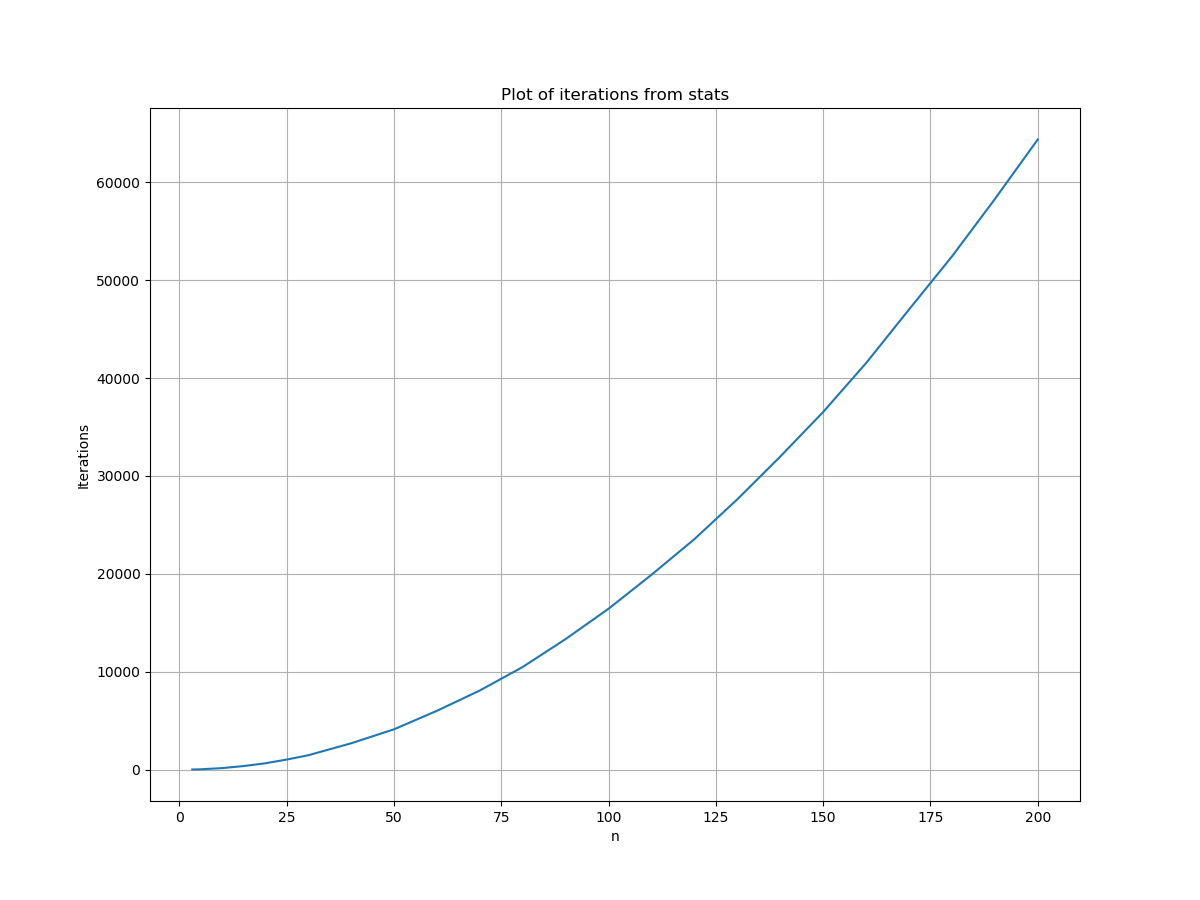
\includegraphics[width = 11cm]{iterations-stats.png}
    %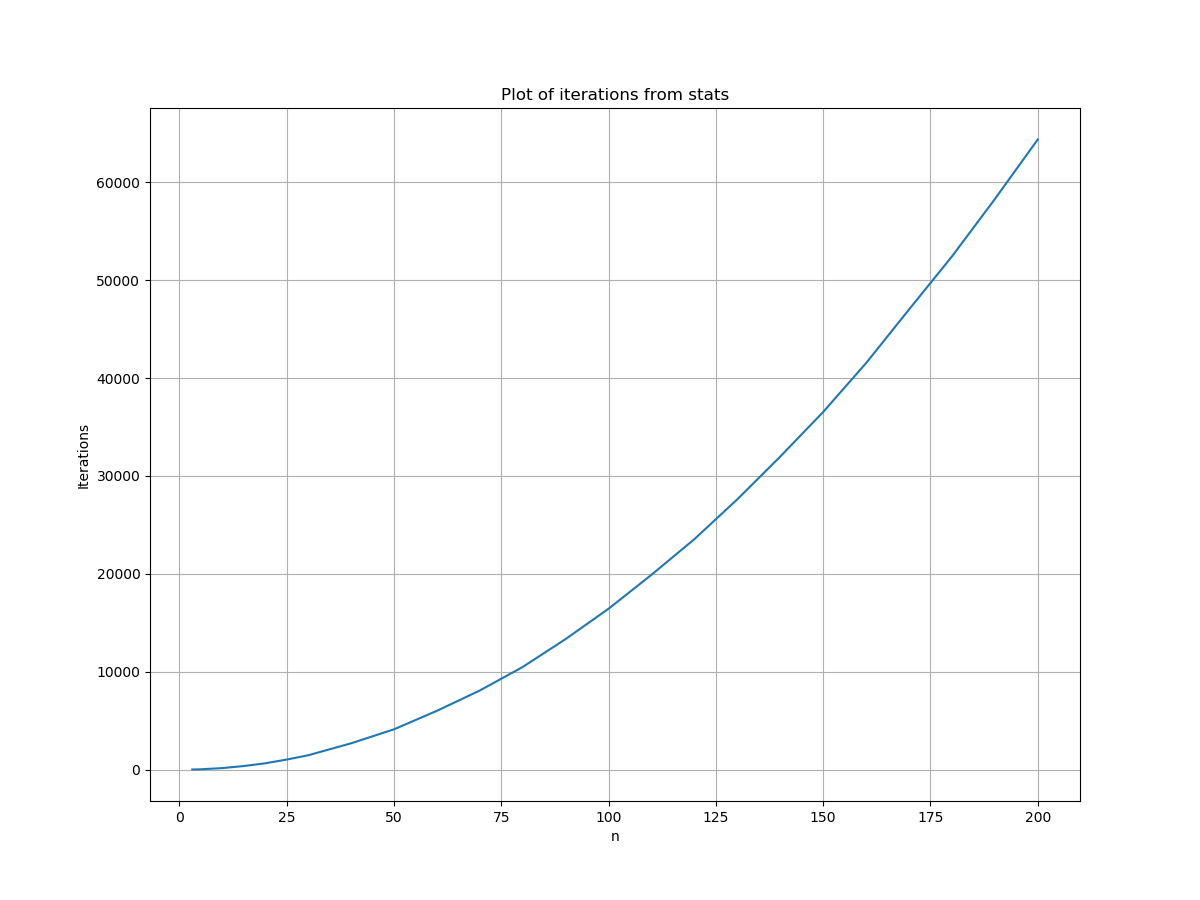
\includegraphics[width = \linewidth]{iterations-stats.png}
  	\caption{The plot of iterations for the Jacobi method as function of the dimension $n$ of the matrix \textbf{A}. }
    \label{fig:iterationspng}
  \end{figure}

  \begin{figure}[ht]
    \centering
    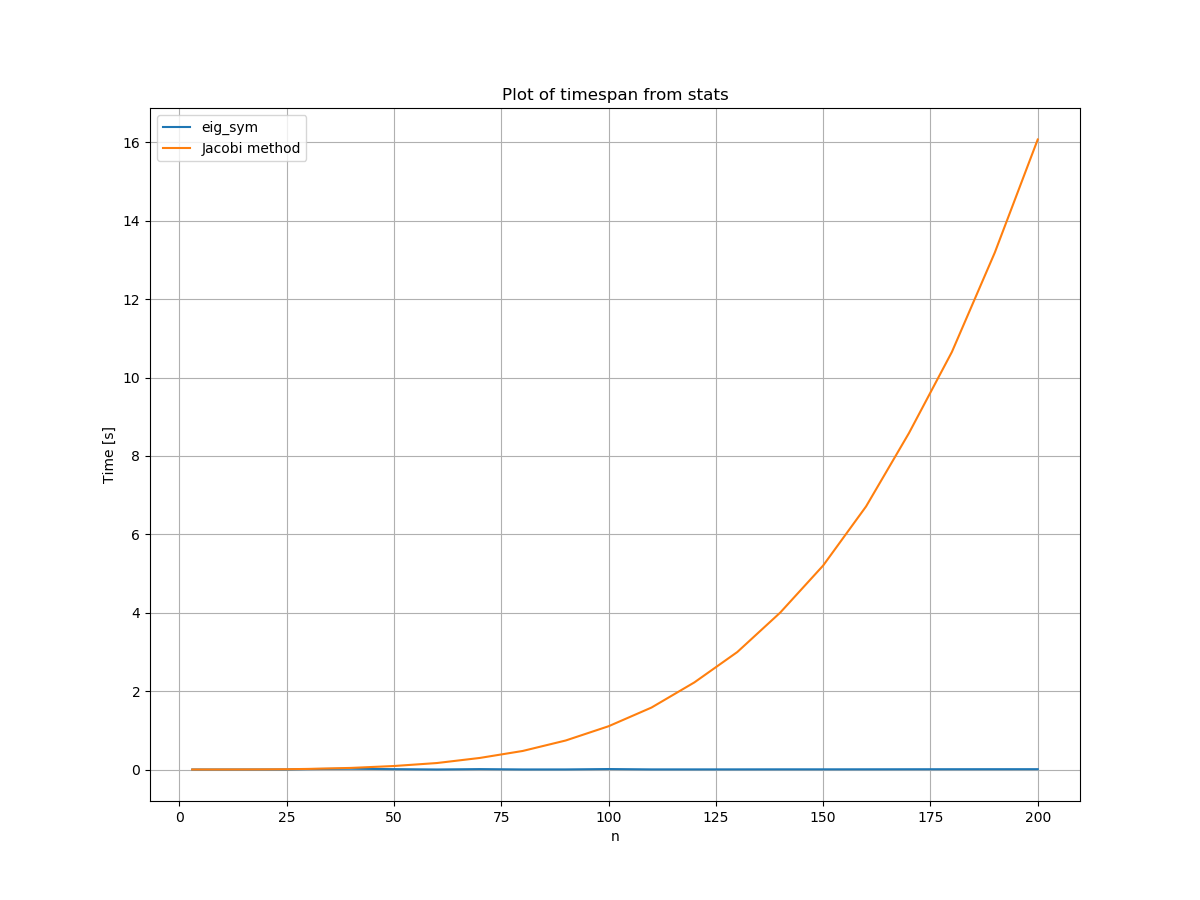
\includegraphics[width = 11cm]{timespan-stats.png}
    %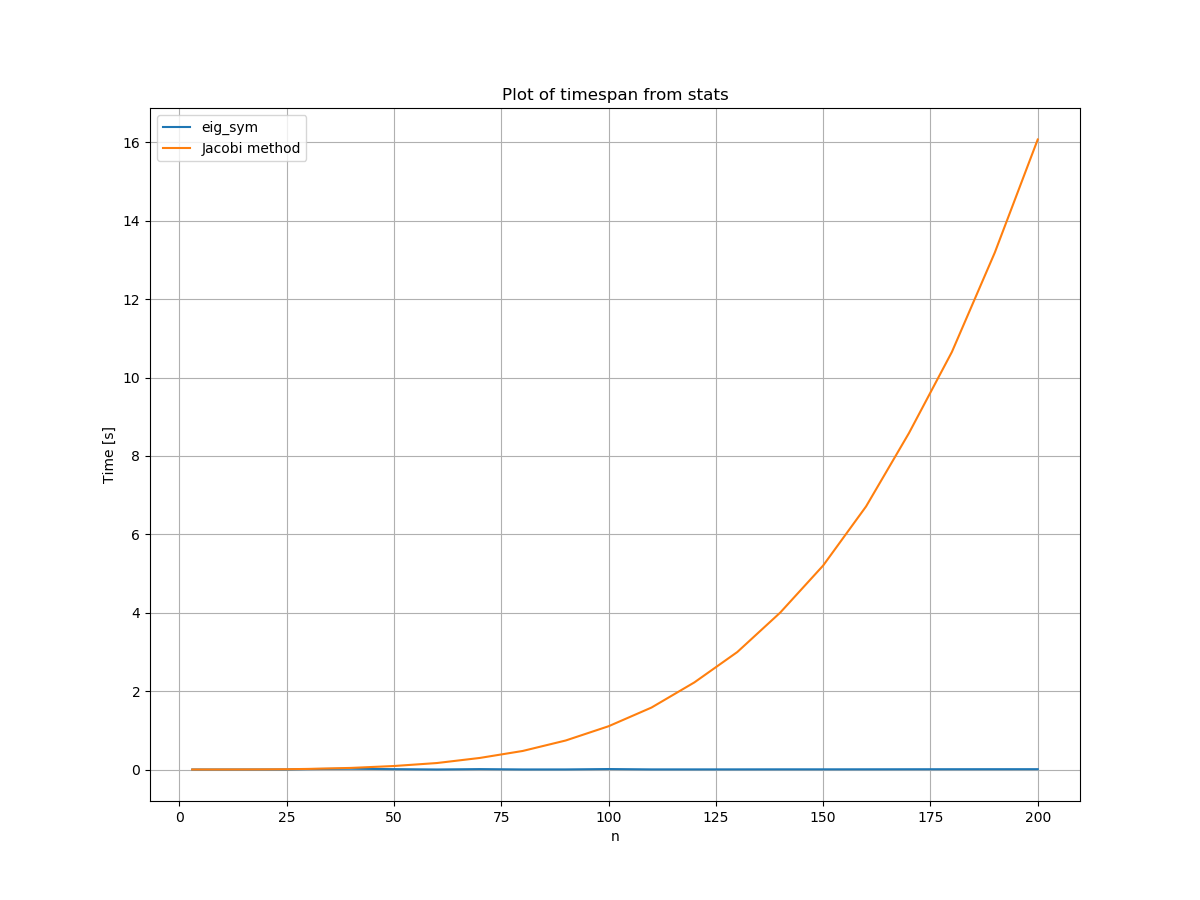
\includegraphics[width = \linewidth]{timespan-stats.png}
    \caption{The plot of the time the function \texttt{eig\_sym} from Armadillo uses and the time Jacobi method uses as functions of the dimension $n$ of the matrix \textbf{A}. }
    \label{fig:timespanpng}
  \end{figure}


\iffalse
  \begin{wrapfigure}{ci}{1.1\linewidth}
    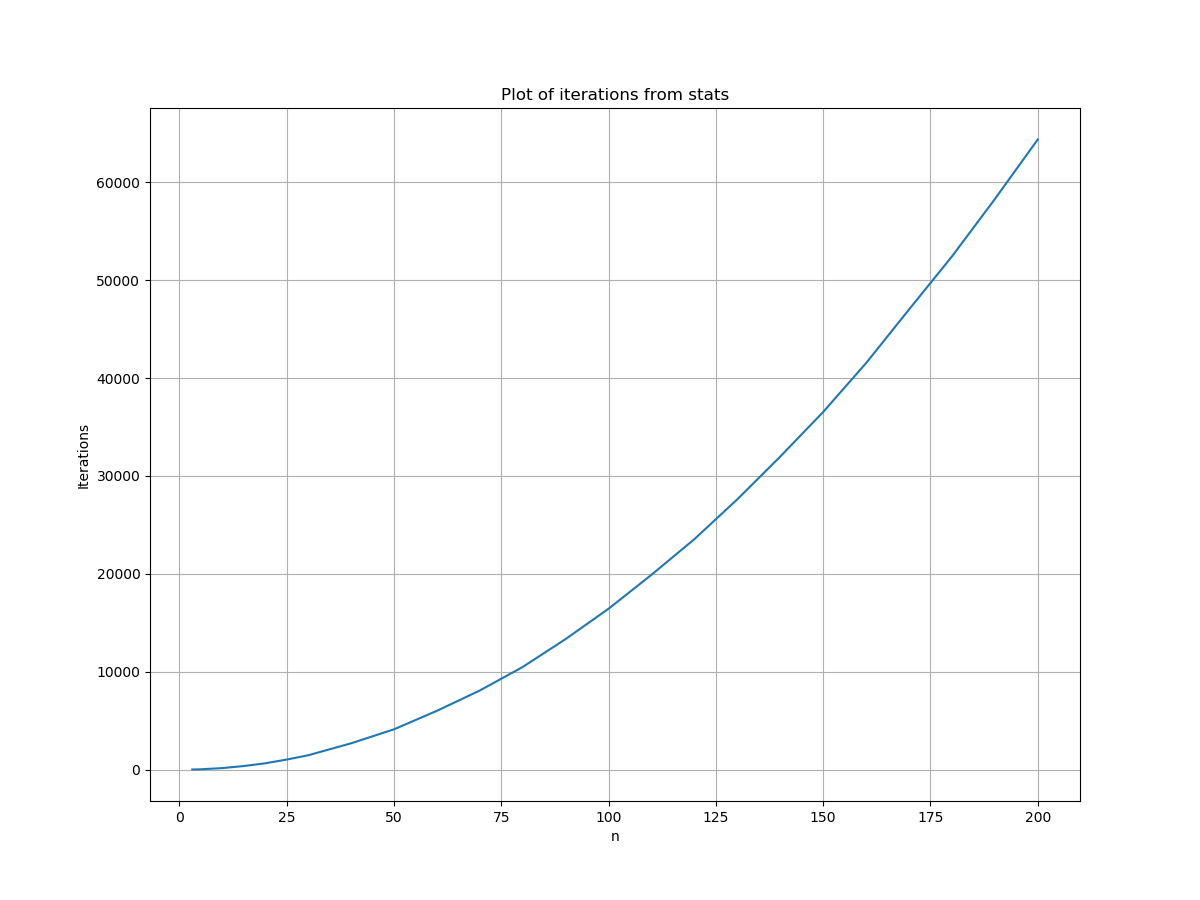
\includegraphics[width=\linewidth]{iterations-stats.png}
    \caption{The plot of iterations for the Jacobi method as function of the dimension $n$ of the matrix \textbf{A}. }
    \label{fig:iterationspngnei}
  \end{wrapfigure}

  \begin{wrapfigure}{li}{1.1\linewidth}
    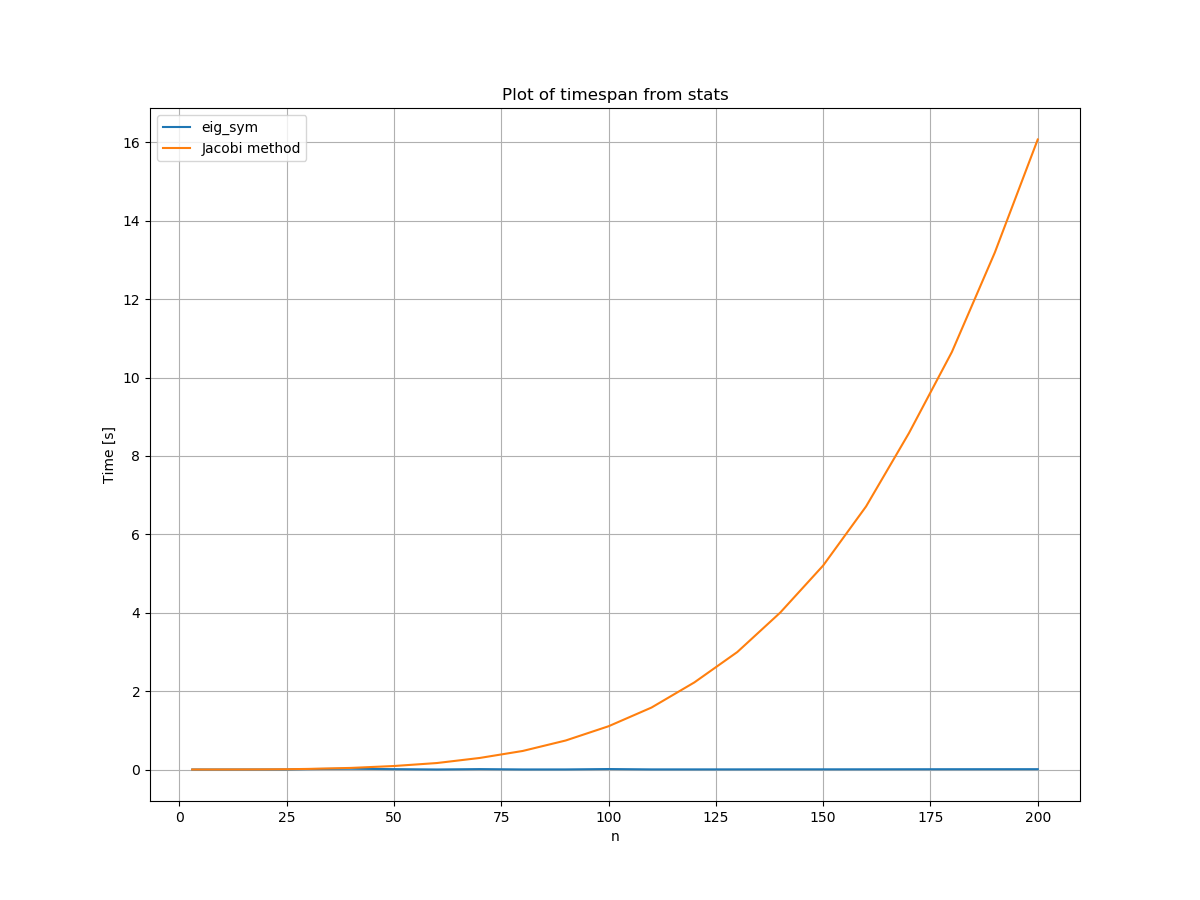
\includegraphics[width=0.5\linewidth]{timespan-stats.png}
    \caption{The plot of the time the function \texttt{eig\_sym} from Armadillo uses and the time Jacobi method uses as functions of the dimension $n$ if the matrix \textbf{A}.}
    \label{fig:timespanpngnei}
  \end{wrapfigure}
\fi

%\clearpage

%\begin{multicols}{2}

  Figure (\ref{fig:iterationspng}) shows that the number of iterations as a function of the dimension $n$ of the matrix has an exponential increase. This means that for larger values of $n$, we need many similarity transformations for our matrix to have all non-diagonal elements become zero. This result coincides with the time difference in the algorithms. We observe that for small matrix-dimensions $n$ our algorithm is sligthly faster than the Armadillo function \texttt{eig\_sym}. When $n$ increases in value, the time used in our algorithm increases exponentially when looking at figure (\ref{fig:timespanpng}). For the biggest given dimension, $n = 200$, our algorithm uses $16$s while \texttt{eig\_sym} uses only $0.008$s. Here we can observe how slow our algorithm is compared to \texttt{eig\_sym}. \\

  %\setlength{\arrayrulewidth}{1mm}
  \setlength{\tabcolsep}{1mm}
  %\renewcommand{\arraystretch}{1.5}

  \begin{table}[ht] \label{tb:harmonic.txt}
    \centering
    \caption{The eigenvalues of the harmonic oscillator for one electron for different integration points $N$ and different dimensionless variables $\rho_{max}$.}
    \vspace{2mm}
    \begin{tabular}{| l c | c c c| }
      \hline
      \multicolumn{1}{| c}{$\rho_{max}$}
      &  \multicolumn{1}{c}{}
      &  \multicolumn{1}{c}{1}
      &  \multicolumn{1}{c}{5}
      &  \multicolumn{1}{c |}{10} \\
      \cline{1-5}
          & 5   & (10.11, 36.49, 72.49, 108.49) & (3.21, 9.07, 14.08, 20.31) & (3.49, 25.72, 45.17, 70.17) \\
          & 50  & (10.17, 39.77, 88.92, 157.47) & (3.23, 7.32, 11.38, 15.43) & (3.45, 7.62, 11.70, 15.70) \\
          & 100 & (10.16, 39.80, 89.10, 158.05) &  (3.11, 7.17, 11.20, 15.23) & (3.23, 7.33, 11.39, 15.42) \\
          $N$ & 150 & (10.16, 39.80, 89.13, 158.16) &  (3.08, 7.11, 11.14, 15.16) & (3.15, 7.22, 11.27, 15.30) \\
          & 200 & (10.16, 39.80, 89.14, 158.20) & (3.06, 7.08, 11.10, 15.12) & (3.11, 7.17, 11.20, 15.23)  \\
          & 300 & (10.15, 39.80, 89.15, 158.22) & (3.04, 7.06, 11.07, 15.09) & (3.08, 7.11, 11.14, 15.16) \\
          & 400 & (10.15, 39.80, 89.15, 158.23) & (3.03, 7.04, 11.05, 15.07) & (3.06, 7.08, 11.10, 15.12) \\
      \cline{1-5}
    \end{tabular}
  \end{table}

  \begin{table}[ht] \label{tb:qdot.txt-omega}
    \centering
    \caption{The eigenvalues of the harmonic oscillator for two electrons where $N = 400$ and $\rho_{max} = 400 $ for varying $\omega_r$.}
    \vspace{2mm}
    \begin{tabular}{| c | c | }
      \hline
      $\omega_r$ & \textrm{Eigenvalues} \\
        \hline
        0.01 & (0.310621, 0.679419, 1.2189, 1.94162) \\
        0.5 & (12.3107, 42.6021, 92.3392, 161.689) \\
        1 & (4.08621, 7.96089, 11.8888, 15.8406) \\
        5 & (7.9323, 37.8442, 57.8296, 77.8307) \\
      \hline
    \end{tabular}
  \end{table}

\newpage

%--------------- Discussion ---------------------------------------
\vspace{1cm}

\section{Discussion} \label{sec:Discussion}

  The number of similarity transformations, also called iterations, needed to reach the desired matrix depends on the dimension $n$. For instance a run of our matrix \textbf{A} given as a $(10 \times 10)$ matrix, there are 154 transformations needed. This number is only exact for this specific run, as it will change for any differences to the matrix, both size and elements. \\

  In the lecture notes it states that for the Jacobi method there is no way to predict the number of transformations needed. See this \href{http://compphysics.github.io/ComputationalPhysics/doc/pub/eigvalues/html/eigvalues.html}{file} under \textit{Discussion for Householder's method for eigenvalues}.

  The Jacobi method is considerably slower for large values of $n$ mainly because the matrix is larger, which means that the algorithm has more elements to rotate and because it has to execute more iterations. The slowness for the Jacobi method is based on when $n$ increases, the algorithm increases the value of some elements, while it decreases the value of others. Consequences of this is that the algorithm has to compute multiple iterations compared to \texttt{eig\_sym} for the same values of $n$.
  Because there is a time difference in the algorithms, we know that \texttt{eig\_sym} does not use the Jacobi method, and is therefore considerably faster. The function most likely observes that the matrix is tridiagonal and finds the easiest solution, based on if-else-statements and different types of eigenpair solvers. When looking at the definition of \texttt{eig\_sym} given on this \href{http://arma.sourceforge.net/docs.html#eig_sym}{website}, the function has an argument \texttt{method} for describing two different methods for using the function. The default option is \texttt{dc}, which stands for \textit{divide-and-conquer}, while the other option is \texttt{std}, which stands for \textit{standard}. The \texttt{dc} method is sligthly faster for smaller matrices, dimension $\tilde 300$ and smaller, but for larger matrices it is considerably faster.
  When testing \texttt{eig\_sym} with both methods for matrices of sizes $n = \{ 1000, 5000, 10000\}$ there is already a notable diffrence for $n = 1000$, where \texttt{dc} is ten times faster than \texttt{std}. Because we compute with matrices of dimension $n = 200$ and smaller, the difference in usage of \texttt{eig\_sym} can be ignored as it gives very similar results. \\

  We can see that changing the frenquency has an impact on the energy of the eigenstates. We can first confirm that our algorithm works by running for $ \omega_r=0.25$, which gives us $1.25$. This is twice that of the tabulated value in the article by M. Taut. They have another scaling which gives them half of ours. \\

  By running for $ \omega_r= \{ 0.01, 0.5, 1, 5 \}$ we can see the difference in values (see \ref{tb:qdot.txt-omega}). We generally have an increasing energy for the ground state (0.3, 12.3, 4.1, 7.9). This makes sense as a higher frequency generally leads to increased energy (think of electromagnetic waves for example). The 12.3 is from $\omega_r=0.5$ and kind-of sticks out. We can imagine that this frecuency resonates weirdly with the system, perhaps in a poor way, giving us the increased energy. \\

  All results in table (\ref{tb:qdot.txt-omega}) have a number of integration points that the analytical results do not posess. In addition our algorithm is incapable of giving the analytic results with four leading digits. This could be from an errror in the indexing, or perhaps a weird compiler in Windows QtCreator. Nevertheless the algorithm gives correct results to an acceptable accuracy.


%---------------Conclusion and perspective---------------------------
\vspace{1cm}

\section{Conclusion and perspective} \label{sec:Conclusion}

Through testing different size matrices the data shows that the Jacobi method is inferior to the methods used by the Armadillo function. What this difference comes from is hard to say for certainty because it was close to impossible to find the methods the Armadillo function used. What can be said for certain is that Jacobi method changes in this case two elements to zero, but also has an effect on other elements in the matrix. A zero element can be changed to a non-zero element. Therefore the method needs to be repeated many times in order to make each element within the epsilon-range of 0. Despite the methods ineffectiveness it did enough to solve all the quantum mechanics problems and one of the advantages of the Jacobi method is that it can solve the eigenvectors of any given matrix. All in all it is a consistent method for solving eigenvalue problems, but the lacking efficiency makes it less viable for big projects where other methods have clearly shown higher potency.

%--------------Appendix---------------------------------------------
\vspace{1cm}

\section{Appendix} \label{sec:Appendix}

\subsection{Assorted data}

Under follows the data in \texttt{stats.txt}.

\begin{verbatim}
  n, iterations, timespan eig_sym, timespan ours
  3, 10, 1.137520e-04, 1.666000e-05
  5, 32, 8.632200e-05, 6.015200e-05
  10, 154, 8.277800e-05, 3.797710e-04
  15, 363, 1.395090e-04, 1.351192e-03
  20, 644, 2.044150e-04, 3.183269e-03
  25, 1025, 2.189260e-04, 7.074493e-03
  30, 1463, 1.089399e-02, 1.494651e-02
  40, 2685, 1.947745e-02, 4.040845e-02
  50, 4115, 8.989085e-03, 8.897613e-02
  60, 6007, 7.917790e-04, 1.650397e-01
  70, 8081, 1.022618e-02, 2.948578e-01
  80, 10487, 1.577296e-03, 4.732270e-01
  90, 13338, 2.079035e-03, 7.397605e-01
  100, 16438, 1.184104e-02, 1.103670e+00
  110, 19905, 2.845618e-03, 1.580353e+00
  120, 23547, 3.005831e-03, 2.222943e+00
  130, 27615, 3.534705e-03, 2.997598e+00
  140, 31981, 4.432247e-03, 4.003528e+00
  150, 36537, 4.577840e-03, 5.204313e+00
  160, 41531, 5.158932e-03, 6.712134e+00
  170, 47005, 6.375916e-03, 8.584403e+00
  180, 52424, 7.180886e-03, 1.065379e+01
  190, 58289, 7.780051e-03, 1.319042e+01
  200, 64379, 8.258574e-03, 1.607514e+01
\end{verbatim}

%------------------------------

\subsection{\texttt{plot\_data.py}}

The program \texttt{plot\_data.py} reads the \texttt{.txt}-file made in \texttt{jacobimethod.cpp} and plots the data. \texttt{jacobimethod.cpp} generates the file \texttt{stats.txt}, which contains the dimension of the matrices, \texttt{n}, the number of iterations, \texttt{i}, the time used for the Armadillo-funtion \texttt{eig\_sym}, \texttt{timespan eig\_sym} and the time used in our algorithm, \texttt{timespan ours}.
\texttt{plot\_data.py} plots the number of iterations needed given by different values of the matrix dimension and it plots the time used as a function of the matrix dimensions. The values in \texttt{stats.txt} is taken from multiple runs of \texttt{jacobimethod.cpp} for different dimensions of the matrices. The figures (\ref{fig:iterationspng}) and (\ref{fig:timespanpng}) are the plots from \texttt{plot\_data.py}.




%\clearpage

%----------------Refrences----------------------------------------
\vspace{1cm}

\section{References} \label{sec:References}

\href{https://github.com/CompPhysics/ComputationalPhysics/blob/master/doc/Projects/2019/Project2/pdf/Project2.pdf}{Link to the PDF for Project 2}. \\

\href{https://github.com/Erikbgram/Fys3150}{Our GitHub-repository}. \\

\href{https://github.com/CompPhysics/ComputationalPhysics/blob/master/doc/Lectures/lectures2015.pdf}{Link to lecture slides in FYS3150 - Computational Physics}. \\

\href{http://arma.sourceforge.net/docs.html#eig_sym}{Offical Armadillo website for documentation of all contents in the library}. \\

\href{https://journals.aps.org/pra/pdf/10.1103/PhysRevA.48.3561}{Analytical results for specific oscillator frequencies}. \\





%----------------Slutten av dokumentet---------------------------------------



%\end{multicols}

\end{document}
